\section{Related Work}

The Skip Lists data structure is introduced by \cite{pugh:90} as a
probabilistic alternative to balanced trees and is shown in
\cite{zachary:BST:2007} to be as elegant as and easier to use than binary search
trees. Such a structure is later employed for self-indexing of inverted lists
in \cite{moffat:96}. Self-indexing inverted list enables a sub-linear
complexity in average when intersecting two inverted lists. \cite{boldi:05}
proposes a way to compress efficiently a Skip Lists directly into an inverted
list and shows that it is possible to achieve a substantial performance
improvement. however by embedding the skips directly into the inverted list
disrupts the values distribution of the list. Indeed block-based compression
methods show performance dependent on the integers distribution.
\cite{chierichetti:08}, the authors introduce a method to place skips
optimally given the knowledge of the query distribution. However the query
distribution can not be known in the use case of Sindice, because of the
diversity of datasets schema it is impossible to create a set of queries that
likely will be run. \cite{messeguer:skiptrees:1997} presents a generalized
Skip Lists data structure for concurrent operations.

\section{Skip Lists}
\label{sec:skiplists}

Skip Lists is a self-indexing structure that builds a sparse index over the
inverted lists and provides fast record lookups. In this section, we first
present the Skip Lists model and its associated search algorithm. We finally
discuss the effect of the probabilistic parameter with respect to the Skip
Lists data structure and search complexity.

\subsection{The Skip Lists Model}

Skip Lists are used to index records in an inverted list at regular interval.
These indexing points, called \emph{synchronization points}, are organized
into a hierarchy of linked lists, where a linked list at level $i+1$ has a
probability $p$ to index a record of the linked list at level $i$. The
probabilistic parameter $p$ is fixed in advance and indicates the
\emph{interval} between each synchronization point at each level. For example
in Figure~\ref{fig:skiplists}, a synchronization point is created every
$\frac{1}{p^1} = 16$ records at level 1, every $\frac{1}{p^2} = 256$ records
at level 2, and so on. In addition to the pointer to the next synchronization
point on a same level, a synchronization point at level $i+1$ has a pointer to
the same synchronization point at level $i$. For example in
Figure~\ref{fig:skiplists}, the first synchronization point at level 3 (i.e.,
for the record 4096) has a pointer to the level 2 which has itself a pointer
to the level 1. This column of synchronization points is called a \emph{tower}.
This hierarchical structure enables to quickly find a given record using a
top-down search strategy.

Given the probabilistic parameter $p$ and the size $n$ of an inverted list, we
can deduce two characteristics of the resulting Skip Lists data structure: 
\begin{enumerate}
\item the expected number of levels
\begin{equation}
L(n)=\left\lfloor \ln_{\frac{1}{p}}(n)\right\rfloor
\label{eq:skiplists-maxlevels}
\end{equation}
\item the size, i.e., the total number of synchronization points is given by
\begin{equation}
S(n)=\sum_{i=1}^{L\left(n\right)}{\left\lfloor n\times p^i \right\rfloor}
\label{eq:skiplists-size}
\end{equation}
which sums up the number of synchronization points expected at each level. 
\end{enumerate}
$L(n)$ sets the maximum number of levels, since \cite{pugh:90} shows that
the probability that it is actually greater is very low.

The number of levels at a synchronization point is fixed according to its
position in the inverted list. If this was set randomly, a level i might not
have the probability of expected synchronization points at $p^i$. This reflects
that the balancing of synchronization points is probabilistic rather than
strictly enforced, thus making the algorithm to build the structure easier than
in balanced trees. For example at the building phase of the Skip Lists in the
Figure~\ref{fig:skiplists}, writing the 256-th record triggers the building of
$L(256)=2$ levels.

\subsection{Search Algorithm}
\label{sec:search-skiplists}

The Skip Lists enables to retrieve an interval containing the
target record and is performed using a top-down strategy. The search within an
interval is discussed in Section~\ref{sec:search-interval}. The search walk
starts at the head of the top list, and performs a linear walk on a level as
long as the target is greater than a synchronization point. The walk goes down
one level if and only if the target is lower than the current synchronisation
point. The search finishes when the current synchronization point is
\begin{inparaenum}[(a)]
\item equal to the target, or
\label{target-equal}
\item on the bottom level and greater than the target.
\label{target-lower}
\end{inparaenum}
The reached interval then contains the target.

The search complexity is defined by the number of steps necessary to find the
interval holding the target. In the worst case, the number of steps at each
level is at most $\frac{1}{p}$ in at most $L(n)$ levels. Consequently, the
search complexity is
\begin{equation}
C_S=\frac{L(n)}{p}
\label{eq:skiplists-complexity}
\end{equation}

The Figure~\ref{fig:skiplists} depicts with a solid line the search path in a
Skip Lists with $p = \frac{1}{16}$ and $L(n)=3$ levels to the record 8195. At
the top of the Skip Lists, we walk to the record 8192. Then we go down to level
1 and stop because the current synchronization point (i.e., the record 8208) is
greater than the target. At this point, we know that the target record is in
the interval directly before the current synchronization point on the inverted
list. The searched record is reached by scanning the records until the target
is found.

\begin{figure}
\centering
\resizebox{0.7\linewidth}{!}{%
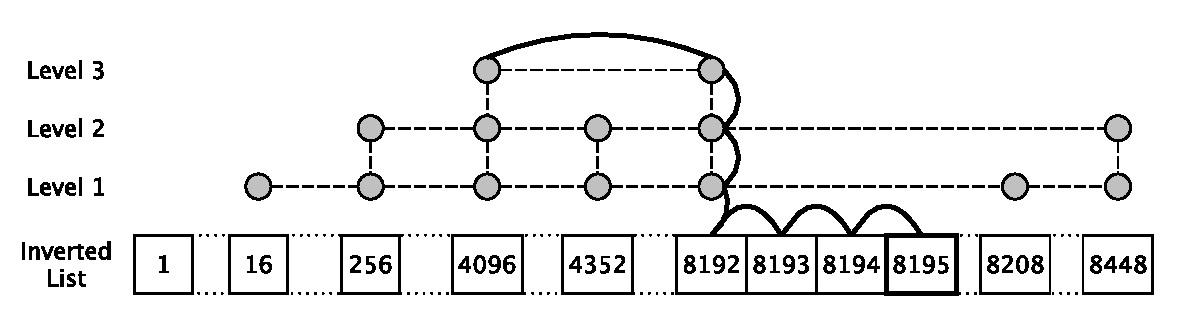
\includegraphics[scale=1]{pics/skiplists}
}%
\caption{Skip Lists with $p=\frac{1}{16}$. Dashed lines denote pointers between
synchronization points. The solid line shows the search path to the record 8195.}
\label{fig:skiplists}
\end{figure}

\section{Implementation}
 
 In this section we present the implementation of the Skip Lists structure as
 found in the open source project Apache Lucene\footnote{Apache Lucene:
 \url{http://lucene.apache.org/}}.
 
\paragraph{Structure}

The structure's data is kept on disk, and as such its implementation is done so
that the cost of IO operations are reduced. Each level of the Skip Lists is
stored as one stream, in order to read continuous data on disk when reading
synchronization points at a same level. The levels are stored one after the
other in reverse order, starting from the top level to level 1. The reverse
order storage of the levels is so that it maps the search algorithm flow, i.e.
we start on the top level, then descend levels to the bottom. The
Figure~\ref{fig:skiplists-impl} depicts the Skip Lists' Lucene implementation
of a synchronization point with 3 levels. The $ID$ refers to the record
identifier needed to advance in the Skip Lists. The \emph{Data} holds
information about the inverted list built upon such as file pointers. For a
same synchronization point such as in the figure, the Data block stores the same
information at each level about the inverted lists (i.e., duplicate data). The
next grey block depicts a file pointer, intern to the Skip Lists. This file
pointer stores the offset of a same synchronization point at the level below.
We can point out that for performance reasons, this file pointer points to the
end of a Data block, so that a duplicate information is not read twice when
descending levels.
 
\begin{figure}
\centering
\resizebox{0.6\linewidth}{!}{%
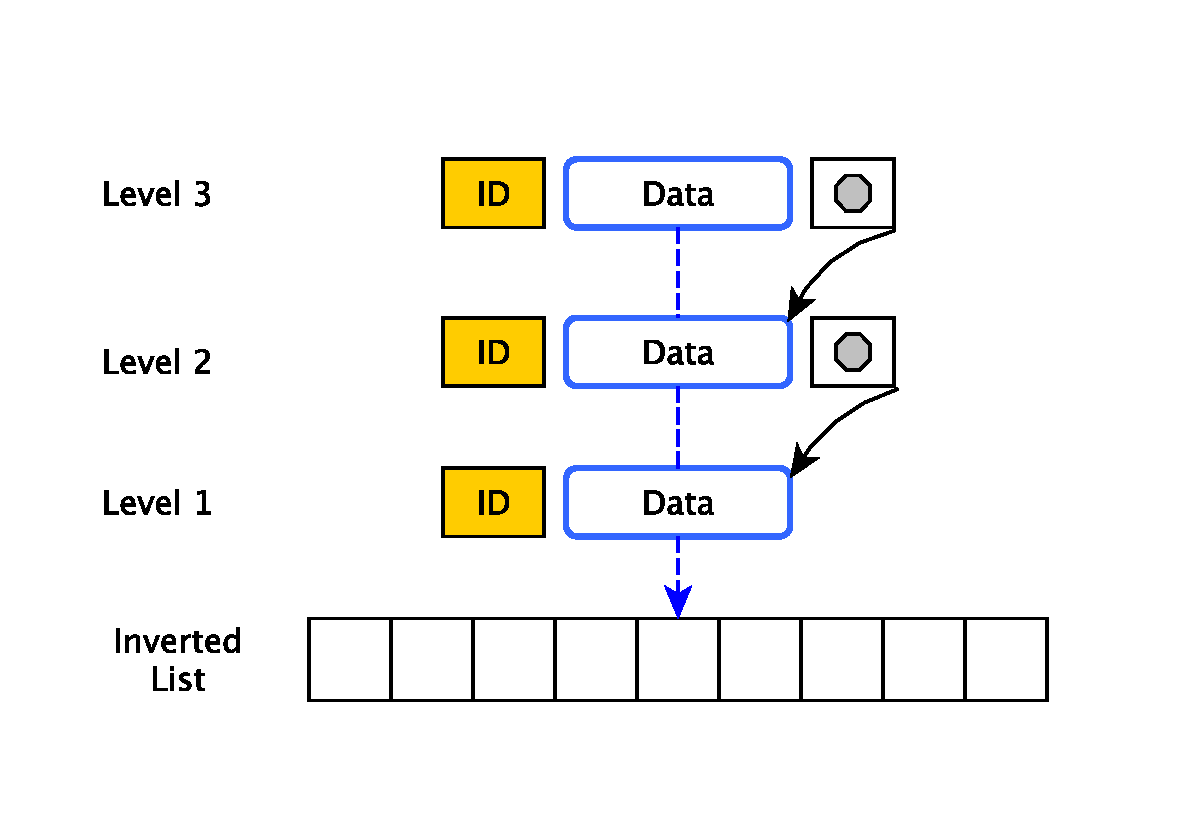
\includegraphics[scale=1]{pics/skiplists-impl}
}%
\caption{Skip Lists structure's implementation.}
\label{fig:skiplists-impl}
\end{figure}

\paragraph{Search algorithm}

The algorithm flow of the Skip Lists is highly optimized by having the less
branching conditions possible in order to maximizes the search throughput.
Given a targeted record that possibly is in the inverted list, the
\emph{\texttt{\#skipTo()}} method returns the interval that would hold it. On
the second line, the levels streams are loaded from disk if not done already.
The lines 4 to 6 walks up the levels as long as the current record identifier
of level i (i.e., stored within the \emph{currentIDs} variable) is lower than
the target. This allows to read only the levels that might skip to the target.
The loop starting at line 8 advances within the Skip Lists, by reading a
synchronization point at level i (line 10) as long as the current identifier is
lower than the target. On lines 12-13 we advance on the stream below to the
synchronization point which is the last being lower than the target.

\vspace{1em}
\begin{lstlisting}[frame=lines,language=Java,numbers=left,caption=Implementation of
the Skip Lists search
algorithm,label=lst:skiplists-search-algo,emph={currentIDs,moveToSynchronizationPoint,readSynchronizationPoint},
emphstyle={\bfseries}]
skipTo(int target)
	loadLevels();
	// Walk up the levels
	int level = 0;
	while (level < MAX_LEVELS - 1 && target > currentIDs[level + 1])
		level++;
	// Search for the interval containing the targeted record
	while (level >= 0) {
		if (target > currentIDs[level])
			readSynchronizationPoint(level)
		else
			moveToSynchronizationPoint(level-1);
			level--;
	}
\end{lstlisting}
